%Just putting something here as a placeholder..(GSL) e
%Not sure what to put here


%%%%%%%%%%%%%%%%%%%%%%%%%%%%%%%%%%%%%%%%%%%%%%%%%%%%%%%%%%%%%%%%%%%%%

\section{Introduction}
\label{sec:intro}


% The truth: I wanted to take paco's D18 course, but I couldn't afford it (both in time and money), so I wanted to do something graphics-y. 
%            It also somehow got into my head that raytracing black holes was something to do, I think maybe paco's students showed me?
% What I will tell people:

% Motivation... why we are doing this? and why is interesting...
Raytracing is a foundational technique in computer graphics, which can be used
to render photorealistic scenes.
A good introduction to the main techniques and practical implementations can be found
in this Ref.\cite{raytracing_in_one_weekend}.
\CMT{maybe describe the basics in 2 or 3 sentences...}
In general this implies expensice proccesses and requires the corresponding aproppiate compute time
as well as complex and sophisticated algorithms.
Their applications range from, geenration of high-quality realistic visualizations
in rendering of movies, animations, and even up to more excotic images of Black Holes,
such as te ones remarkably done for the BH reciding at the center of the galaxy M87 \cite{M87_EHT_i},
which have captivated the minds of millions.
Since we have well established the theory and equations for describing the trajectories of light rays around a black hole, it is natural to try to use a ray tracer to render a scene within this geometry which ultimately results in a particular distortion applied to the general techniques.
%Raytracing is a foundational technique in Computer Graphics, which can be used to render photorealistic scenes with the proper compute time, and images of Black Holes, such as M87 \cite{M87_EHT_i}, have captivated the minds of millions. Since we have well established equations for describing the trajectories of light rays around a black hole, it is natural to try to use a ray tracer to render a scene with this distortion applied.

We should emphasize that there exist a large variety of raytracers implementations already 
\cite{sharma2023mahakalapythonbasedmodularraytracing,imbens2023graphicalprocessinggeodesicpropagation,10.2312:vmv.20221208,10.2312/EGPGV/EGPGV12/051-060,7539599_OSPRay,James_2015}
and even with direct astrophysical applications such as the rendering of black hole surroundings.
However, our approach seek to highlight some specific features:
i) its open-source implementation;
ii) the minimalistic and simplistic technicality, i.e. by tackling
mostly the actual mathematical problem using specialized libraries
to solve the governing differential equation of the problem;
iii) the proximity to implement this in a farely efficient and high-performing
way by employing standards in shared-memory and distributed-memory paradigms;
and iv) the hardware agnostic approach, i.e. not depending on specialized hardware, accelerators or GPUs which one could argue would be much better suited for tackling this type of problems.

In order to model a simple black hole scenario, we can use the Schwarzschild metric \cite{schw_soln-2007}.
This models black holes which, among other properties, are non-spinning and not charged,
meaning that their deformation of the trajectories of light rays do not depend on the angle of approach.
%\cite{federov2019notes}
It has been well established \cite{gravitation-mtw} that the equation,
\begin{equation}
	u'' - u = 3 M u^2
	\label{eq:Sch-light-ray}
\end{equation}
relates the trajectory of a light ray to the mass $M$ of a black hole, from the Schwarzschild metric;
where $u$ represents $1/r$, being $r$ the Euclidean distance of a point on the light ray to the black hole center.
$u$ is differentiated with respect to $\phi$, the azimuthal angle between the point and the black hole origin.
\CMT{we may need a diagram here}
After providing initial conditions,  it is possible to solve Eq.(\ref{eq:Sch-light-ray}) and trace the entire trajectory of the ray with high fidelity.
Notably, this equation is modeled in 2d-spherical coordinates, meaning, if we want to use this equation to analyze light rays in 3D space, we need to find a way to find an equivalent ray that our equation models, and use the 2D ray to find the 3D ray's trajectory.

After being able to compute the trajectory of individual rays, we can use these rays to generate a full image using ray tracing. Ray tracers render a simulated scene by casting light rays from a simulated camera, and computing what objects in the scene would be visible to that ray. If a particular camera would produce an image of let's say $1920 \times 1080$ pixels, we could build the image that camera would record by casting a light ray through each pixel. Because ray tracing's unit of perception is how simulated light rays interact with a simulated scene, it is a natural choice for simulations which involve the bending or distortion of light.

\CMT{Some discussion of other papers can be made here}

\CMT{Can improve flow here}
This paper is organized as follows:
in Sec.~\ref{sec:intro} we present the physical problem of tracing rays of light in the presence of a black hole;
in Sec.~\ref{sec:impl} we describe the methods implemented and used to tackle this problem;
in Sec.~\ref{sec:results} we discuss our results and compare to other related works;
and finally in Sec.~\ref{sec:disc} and ~\ref{sec:concl} we present our findings and comment
on possible future extensions to this work.

Having given an introduction in Sec.~\ref{sec:intro} to the problem, we will proceed in Sec.~\ref{sec:impl} to describe our implementation approach, followed by results in  Sec.~\ref{sec:results} and a discussion in Sec.~\ref{sec:disc} and ~\ref{sec:concl}.


%%%%%%%%%%%%%%%%%%%%%%%%%%%%%%%%%%%%%%%%%%%%%%%%%%%%%%%%%%%%%%%%%%%%%

\section{Implementation}
\label{sec:impl}


\subsection{Approximating the trajectory of a light ray as a piecewise function}
While the fundamental idea of taking a ray tracer and modifying it so that light rays are distorted is sound, the implementation of such an idea is fraught with difficulty. The first major challenge is that ray tracers need linear equations to be able to compute object intersection in a scene. This means we need to find a way to describe our light ray as a piecewise-defined set of linear equations. We found the best way to do this was to compute discrete points on the light ray, and compute intersection using the line segments defined by said points. 


\subsection{Using GSL for ODE approximation}
As for how to compute these segments, the GNU Scientific Library's (GSL) suite \cite{10.5555/1538674} of ODE approximation tools found significant utility. GSL allows us to define our equations as C functions, and our particular ray by a set of initial conditions. From there, we can use GSL to compute a series of discrete points on the ray governed by a timestep of our choosing. For initial conditions, we need to describe,in 2D spherical coordinates, an initial point on the ray and a single successor point, which was computed using the linear direction, as we are casting rays far from the black hole's influence. As for the timestep (as it is commonly known in the GSL documentation), we allowed program users to control the "epsilon" \CMT{this requires a defintion! -- ie what is epsilon} of the simulation, with lower epsilon values resulting in more accurate trajectories, but also requiring more computed points. 

\subsection{Ensuring even spacing of computed points}
To compute the next point on a light ray `epsilon` distance away, we would compute, using the Euclidean metric, the light ray's path with no distortion. In spherical coordinates, this allows us to compute the azimuthal angle from the black hole's origin. We can feed this updated azimuthal angle into GSL, and it will return the distance of the ray from the origin of the black hole. In effect, GSL behaves as a function from azimuthal angle to distance, allowing us to compute the needed points in 2D space. See ~\ref{fig:one} for an example of how these paths are computed.   \TODO{Is there a better way to explain this?}
\begin{figure}[h]
  \centering
  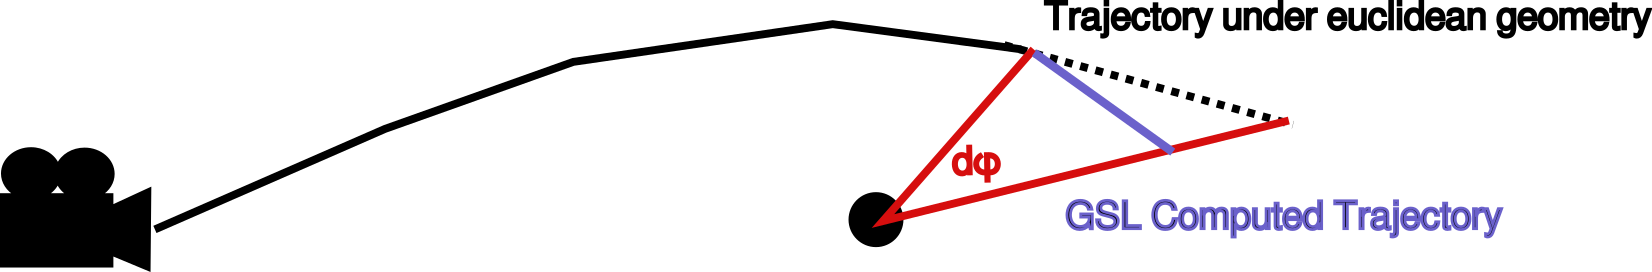
\includegraphics[width=.65\linewidth]{nextpoint}
  \caption{\TODO{HI}: Franklin Model D roadster. Photograph by Harris \&
    Ewing, Inc. [Public domain], via Wikimedia Commons. (\url{https://goo.gl/VLCRBB}).
	\TODO{We need a much better figure here!}}
	\Description{A woman and a girl in white dresses sit in an open car.}
  \label{fig:one}
\end{figure}


\subsection{Relating our 2-variable equation to 3D space.}
As noted earlier though, we cannot use the trajectories of rays in 2D space to render a 3D scene, meaning we need to find a way to find a 1-to-1 relationship between a subset of 3D rays and 2D rays. The solution here was to recognize that we could apply a combination of axis rotations and axis relabeling to complete the correlation. If the "origin" of the light ray, and the origin of the black hole are both located on the z=0 axis, as is the case for our 3D scenes, we can rotate our ray around the z axis until the ray's direction vector has incline $ \pi / 2 $ with respect to the black hole origin, meaning the ray has no spherical incline. At this point, the y component of the ray's origin and direction will both be zero, meaning we have reduced our 3D ray to 2D. From here, we can easily convert to spherical coordinates for use with GSL. Since this process is invertible, we have now found a way to use GSL to trace the trajectory of light rays in 3D using an equation of two variables.


\subsection{Image and scene handling}
%As astronomical images can be of quite high resolution, and the effects of gravitational lensing, when viewed against a high quality background image, are more significant, we wanted to ensure our renderer would work well, even in the case of large images. To accommodate this, we allowed for different MPI processes to load different portions of the image
Image and scene handling was done both with JPEG and with PPM support. For JPEG support, Boost's GIL \CMT{this requires a ref} (And consequently libjpeg) was used, and for PPM support, a custom parser was written. Both of these parsers rely on loading the entire image into memory, which has the advantage of quick pixel access, at the cost of potentially loading a lot of unused pixel data into memory. For moderately sized images, this is an appropriate tradeoff, however, for very large astronomical images, this could quickly become a problem, especially as the size of an image (Plus whatever memory is needed for rendering) eclipses the available RAM. To deal with this, future implementations could apply a number of techniques:
1. Refuse to load the image into memory, instead relying on an `fseek+fread` style implementation, which is likely to perform well on SSD storage, but poorly over the network.
2. Decompose the image, and have each process store a portion in memory, at the cost of having to exchange pixels when a light ray "misses" our portion of the image. This strategy, if poorly optimized, could result in horrible performance, as it's quite difficult to predict the trajectories of an arbitrary light ray in advance, meaning we are likely to miss our loaded portion of the image. This could easily yield a network bottleneck.
3. Load portions of the image that are relevant to our render only. This is somewhat of a balance of the previous two approaches, at the cost of additional complexity. 


\subsection{Domain Decomposition}
The essential element of speeding up a problem with Message Passing Interface (MPI) \cite{mpi41} is often to attempt to decompose the problem space into subproblems which can be computed on an individual node. In our case, our problem space is the image we are attempting to render. The most simple solution is to decompose along the scanlines, and render distinct scanlines on distinct nodes. In effect, one would attempt to assign a "band" to each process to render against. As a note, care must be taken to make sure that each process gets a relatively even number of rows, as if one simply divides the number of rows by the number of cores, and assigns it to each process, you are often left with a large remainder assigned to a single process that significantly slows down the speed of computation.

The downside of domain decomposition is that we now have separate bands rendered on separate processes. There are two potential variant implementations. One is to have the "child" processes send their rendered data to a single "parent"/"root" node, which outputs a single image. This is quite convenient for testing, as there is no work required to reassemble the image after rendering. The downside of this is that sending uncompressed pixel data across the network could be quite slow if one is rendering a large scene. To fix this, one could have each process write its "band" to a file, and recombine the images into a large scene later. If image output is done in PPM, this recombination is quite simple, and could likely even be done by a couple clever invocations of `cat`, `head`, and `tail`.


\subsection{Use of OpenMP}
In the context of a single band, it is quite easy to use OpenMP \cite{660313_OMP} to accellerate rendering, as the problem can be decomposed along the individual scanlines. This was quite helpful, as MPI was best used to distribute the problem across nodes, and OpenMP was useful for distributing the problem across cores.
Additionally, as shown in Sec.~\ref{sec:results}, OpenMP threads scale significantly better than MPI processes, meaning we would like to take advantage of the increased performance wherever possible.


\subsection{Code Availability}
Based on all the elements described in the previous sections,
we developed an open source code in C which is available in the following
GitHub repository
	\TODO{add repo}


%%%%%%%%%%%%%%%%%%%%%%%%%%%%%%%%%%%%%%%%%%%%%%%%%%%%%%%%%%%%%%%%%%%%%


\section{Results}
\label{sec:results}

\subsection{A selection of renders}

This section includes results of images rendered with the raytracer. The background images for these renders were taken from NASA's SVS. With both images, it is easy to see the effects of gravitational lensing, as well as the clear Einstein ring. 


% TODO: Cite eagle galaxy image.
\begin{figure}[h]
  \centering
  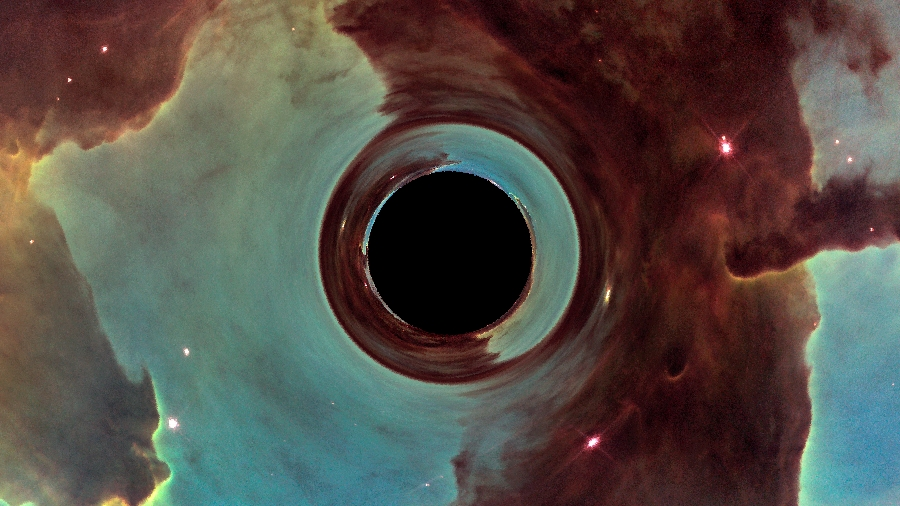
\includegraphics[width=0.8\linewidth]{eagle_render}
  \caption{\TODO{HI}: ....}
    \Description{A woman and a girl in white dresses sit in an open car.}
    \label{fig:eagle}
\end{figure}

%TODO: Cite https://svs.gsfc.nasa.gov/4851/ (Was edited to raise the exposure)
\begin{figure}[h]
  \centering
  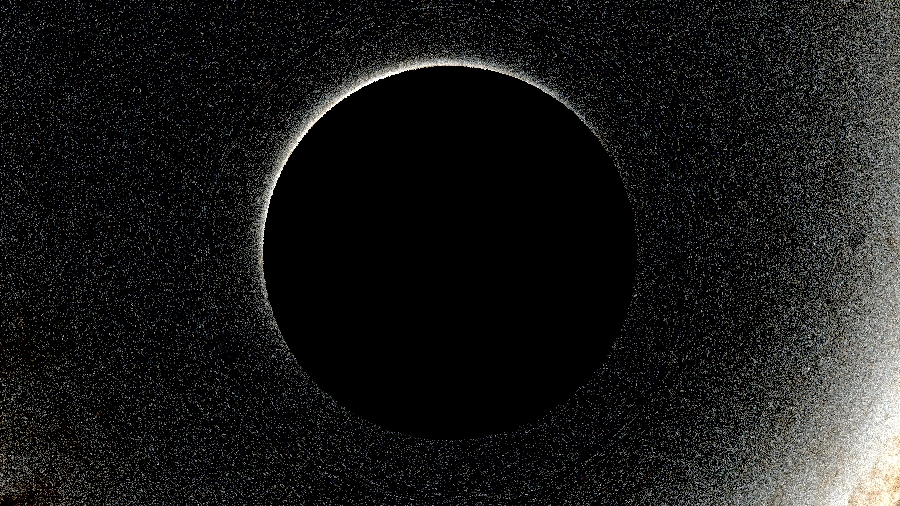
\includegraphics[width=\linewidth]{starry_render}
  \caption{\TODO{HI}: ...}
    \Description{A woman and a girl in white dresses sit in an open car.}
    \label{fig:starry}
\end{figure}




\subsection{Scaling analysis}

With this project, one can attempt to scale along many different axis. You can increase the size of the background image to stress image parsing, you can increase the number of rendered pixels, you can decrease epsilon, yielding to more calls into GSL, or you can increase samples-per-pixel which controls antialiasing. For weak scaling, you can also scale by adding more nodes, or by adding more cores. 

When increasing the size of the background image, this increases the time spent outside the parallel region, as the background image has to be parsed by each process, which is likely to take the same amount of time per node. As such, it does not present significant interest for scaling analysis.

Decreasing epsilon is an interesting scaling parameter, as it is responsible for some of the fidelity of a rendered image. The challenge is that it is hard to be sure how decreasing/increasing epsilon will impact the amount of time needed for a GSL call, which makes it an interesting parameter.

We believe though, that the main parameters of interest are number of rendered pixels, and the number of cores used (across both multiple nodes and single nodes). For testing this kind of scaling without increasing the number of pixels in the scene, antialiasing level could be turned up.

\TODO{When reporting results for the scaling analysis and profiling, we should mention where the runs where done -- i.e. the Niagara supercomputer \cite{10.1145/3332186.3332195}}

\begin{figure*}[h]
  \centering
  \begin{minipage}{0.45\linewidth}
      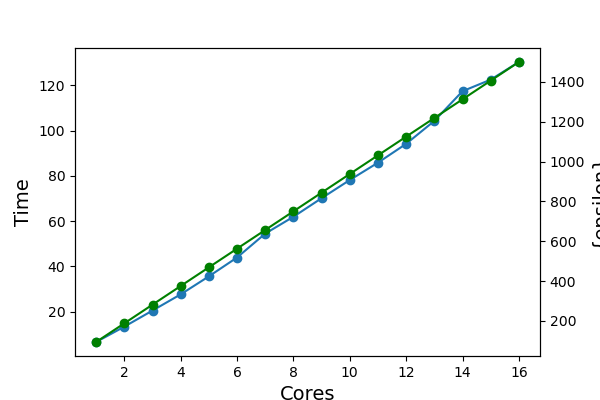
\includegraphics[width=\linewidth]{omp_weak2.out}
      \caption{\TODO{HI}: omp weak 2}        \Description{Weak scaling analysis relating omp thread count, time required for computation, and image width}
        \label{fig:omp_weak2}
    \end{minipage}
  \hspace{.05\linewidth}
 \begin{minipage}{0.45\linewidth}
  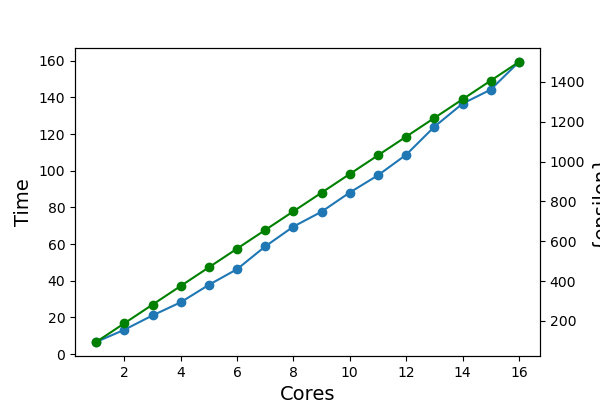
\includegraphics[width=\linewidth]{mpi_weak2.out}
 \caption{\TODO{HI}: mpi weak2 }
    \Description{Weak scaling analysis relating mpi process count, time required for computation, and image width}
    \label{fig:mpi_weak2}
    \end{minipage}
  \begin{minipage}{0.45\linewidth}
      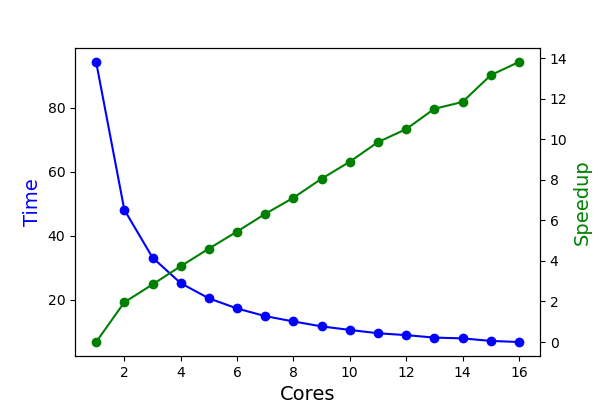
\includegraphics[width=\linewidth]{mpi_strong.out}
      \caption{\TODO{HI}: mpi strong\&
        Ewing, Inc. [Public domain], via Wikimedia
        Commons. (\url{https://goo.gl/VLCRBB}).}
        \Description{Weak scaling analysis relating omp thread count, time required for computation, and image width}
        \label{fig:mpi_strong}
    \end{minipage}
  \hspace{.05\linewidth}
 \begin{minipage}{0.45\linewidth}
  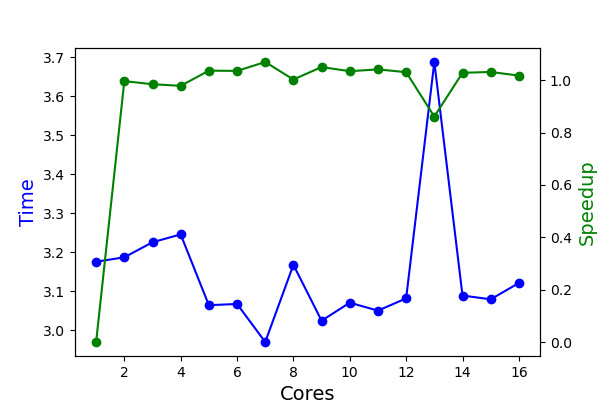
\includegraphics[width=\linewidth]{omp_strong.out}
  \caption{\TODO{HI}: omp strong \&
    Ewing, Inc. [Public domain], via Wikimedia
    Commons. (\url{https://goo.gl/VLCRBB}).}
    \Description{Weak scaling analysis relating mpi process count, time required for computation, and image width}
    \label{fig:omp_strong}
    \end{minipage}
\end{figure*}

From this figure, one can see that, at 16 cores and maximum image width, OpenMP outperforms MPI by around 40 seconds. This is likely explained by the fact that the MPI implementation relies on exchanging pixel data after computations are performed, which is likely to scale poorly with core count. MPI and OpenMP are significantly more competitive at lower core counts.


From Figures ~\ref{fig:omp_weak2} and ~\ref{fig:mpi_weak2}, one can see that, at 16 cores and maximum image width, OMP outperforms MPI by around 20 seconds. This is likely explained by the fact that the MPI implementation relies on exchanging pixel data after computations are performed, which is likely to scale poorly with core count. MPI and OMP are significantly more competative at lower core counts.


\begin{figure}[h]
  \centering
  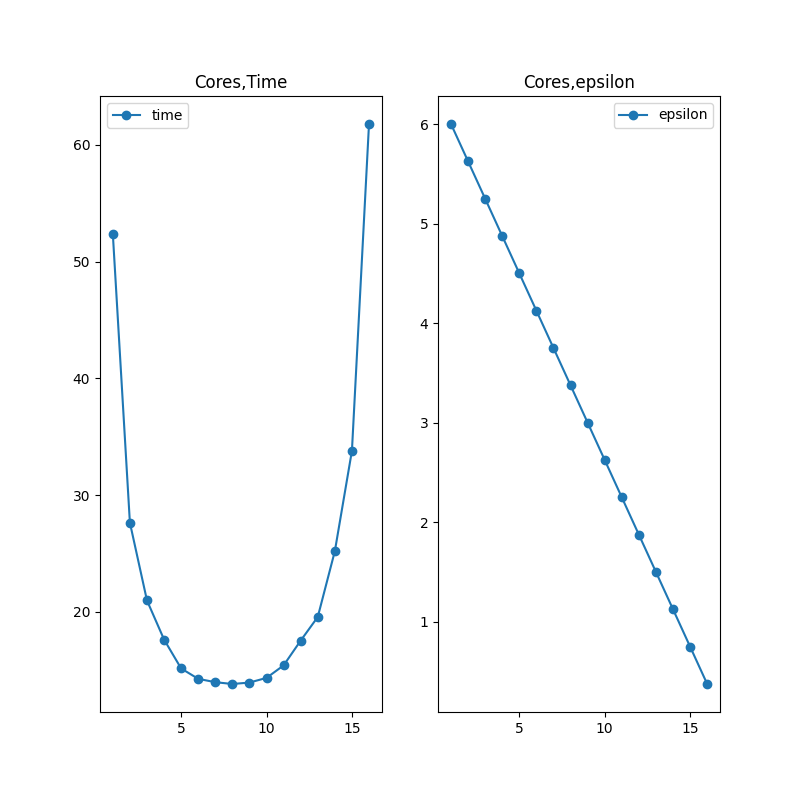
\includegraphics[width=0.55\linewidth]{omp_weak.out}
  \caption{\TODO{HI}: Franklin Model D roadster. Photograph by Harris \&
    Ewing, Inc. [Public domain], via Wikimedia
    Commons. (\url{https://goo.gl/VLCRBB}).}
    \Description{Weak scaling analysis relating omp thread count, time required for computation, and epsilon value. }
    \label{fig:omp_weak}
\end{figure}

\TODO{Are these results legit???}

Interestingly, as observed by Figure ~\ref{fig:omp_weak} decreasing epsilon results in less time complexity, before increasing required time sharply. An epsilon value of about 2-3 results in the best performance.


\CMT{I will fix the fact that I outperformed the ideal, thats bogus}


%%%%%%%%%%%%%%%%%%%%%%%%%%%%%%%%%%%%%%%%%%%%%%%%%%%%%%%%%%%%%%%%%%%%%

\section{Discussion}
\label{sec:disc}

\subsection{Educational Value}


% TODO: Preferred title here?
This raytracer was originally developed for educational purposes in the context of Marcelo Ponce's course CSCD71. As a project, it combines physics simulations (both through the use of a raytracer, and through the simulation of gravitational distortion), ODE approximation with GSL, path stenciling, image/file parsing (esp. at large scale), parallel and distributed computing with MPI and OpenMP, domain decomposition, as well as providing a bountiful quantity of variant implementations, while being of low-enough difficulty to be completed in a few weeks (with great difficulty). The result of which is the ability to render pretty images. In particular, the project would provide potential students an excellent opportunity to learn the practical use of GSL/ODE approximation in a realistic context. The impact is felt in 3 areas:

1. Attempting to set up this particular system is theoretically easy and practically quite difficult. The initial conditions are not obvious. GSL asks for an initial radius, initial angle, and the derivative of the radius with respect to azimuthal angle. Unfortunately, it is not possible to find this derivative without an equation that models the trajectory of light rays, which is the equation we were trying to approximate in the first place! Solving this chicken-and-egg problem is a great educational experience, and forces one to consider more deeply the significance of the parameters given to GSL. 
% (TODO: mention that debugging is hell?)

2. Using GSL for course analysis is a nonstandard application. One key detail of the project is that we need to restrict the number of points GSL returns, while keeping the distance between points relatively even. (TODO: future work: dynamic spacing based off of distortion). The way this challenge was solved was by approximating the angle between the black hole on a line of potential future points, as described earlier, and having the GSL driver stencil the equation until it reaches said line. Idk some closer sentence.

3. The problem of relating the 2D ray-trajectory equation to a 3D scene has no readily available solutions. As such, it challenges potential students to think deeply about the problem, and to come up with original solutions.

Beyond the challenges associated with GSL, this project's requirement of parallel image processing provides an opportunity to learn how to process, parse, and generate large images in parallel. In particular, handling the case where the total handled image size is larger than system memory can yield many variant implementations with considerable performance differences and technical complexity. 

Finally, this project provides an opportunity to practice domain decomposition techniques in a practical setting. %TODO: not sure what else to add here..


\subsection{General Applicability}
One interesting aspect of this design is it's general applicability. Variations of this technique can be used to render any sort of image under light distortion specified by a differential equation. In effect, any distortion function could be input into the ray tracer, and an image modeled under that distortion could be output. In the same line, this technique could be used to render images under the Kerr metric.
% TODO: Forgetting what else is good to put here...


\subsection{Performance Tuning}
There is plenty of room for optimization on top of this ray tracer. A good place to start is that we could get away with calling into GSL significantly fewer times. When the light ray is far from the black hole, we can assume that the distortion is near zero, and thus, that we can simply compute the ray trajectory using Euclidean geometry. With certain settings, approximately 50\% of the ray tracer's runtime is spent inside GSL. Most of this time could be eliminated, resulting in much better performance. 


%\subsection {A better ray tracer}
%This section could discuss possible improvements made to the ray tracer to get better images, more features, etcs


%\subsection {Multiple black holes}
%Can discuss attempting to trace multiple black holes in the same image.


%%%%%%%%%%%%%%%%%%%%%%%%%%%%%%%%%%%%%%%%%%%%%%%%%%%%%%%%%%%%%%%%%%%%%

\section{Conclusions}
\label{sec:concl}

Gravitational lensing is a beautiful phenomenon, both when witnessed from space, and when digitally rendered. This paper explored a relatively simple method for creating a ray traced image which shows gravitational lensing, and how to accelerate the process using shared and distributed memory computing. Additionally, these types of projects lend themselves well to teaching and education, both with regards to general scientific computing techniques, and to HPC techniques.

% TODO: Credit Ray Tracing in One Weekend somewhere...

%%%%%%%%%%%%%%%%%%%%%%%%%%%%%%%%%%%%%%%%%%%%%%%%%%%%%%%%%%%%%%%%%%%%%
